\documentclass[preprint,11pt,authoryear]{elsarticle}
\usepackage[T1]{fontenc}
\usepackage[utf8]{inputenc}
\usepackage{lmodern,microtype,amsmath,amssymb,amsthm,mathtools}
\usepackage{graphicx,booktabs,longtable,array,enumitem,placeins,needspace}
\usepackage[hidelinks]{hyperref}
\usepackage[margin=1in]{geometry}
\newtheorem{theorem}{Theorem}
\newtheorem{proposition}[theorem]{Proposition}
\newtheorem{corollary}[theorem]{Corollary}
\theoremstyle{definition}
\newtheorem{definition}[theorem]{Definition}
\theoremstyle{remark}
\newtheorem{remark}[theorem]{Remark}
\newcommand{\Pbb}{\mathbb P}
\newcommand{\Ebb}{\mathbb E}
\newcommand{\ind}{\mathbf 1}
\newcommand{\Sprof}{\mathcal S}
\newcommand{\Cset}{\mathcal C}
\newcommand{\Eset}{\mathcal E}
\newcommand{\Thset}{\Theta}
\newcommand{\ud}{u^\dagger}
\newcommand{\td}{\theta^\dagger}
\newcommand{\TU}{\theta_U}
\newcommand{\KL}{D_{\mathrm{KL}}}
\newcommand{\draftadmin}[1]{\textbf{[#1]}}
\setlength{\emergencystretch}{2em}

\journal{Computational Statistics \& Data Analysis}
\hypersetup{pdftitle={TrajCert: Sharp risk identification and anytime-valid certification with informative outcome-resolution paths},pdfauthor={Salaheddine Naslouby, Mohamed Lachgar, Hamid Hrimech},pdfsubject={Partial identification and anytime-valid risk certification},pdfkeywords={partial identification, informative verification, mutual information, confidence sequences}}
\makeatletter
\def\ps@pprintTitle{\let\@oddhead\@empty\let\@evenhead\@empty\def\@oddfoot{\hfil\thepage\hfil}\let\@evenfoot\@oddfoot}
\makeatother
\renewcommand{\topfraction}{0.92}
\renewcommand{\textfraction}{0.07}
\renewcommand{\floatpagefraction}{0.70}
\renewcommand{\bibfont}{\small}
\setlength{\bibsep}{2pt plus 1pt minus 1pt}
\begin{document}
\begin{frontmatter}
\title{TrajCert: Sharp risk identification and anytime-valid certification with informative outcome-resolution paths}
\author[aff1]{Salaheddine Naslouby\corref{cor1}\fnref{orcid1}}
\ead{naslouby.salahe@gmail.com}
\author[aff2]{Mohamed Lachgar}
\ead{m.lachgar@uca.ac.ma}
\author[aff1]{Hamid Hrimech}
\ead{hamid.hrimech@uhp.ac.ma}
\cortext[cor1]{Corresponding author.}
\fntext[orcid1]{ORCID: \href{https://orcid.org/0009-0002-7295-7816}{0009-0002-7295-7816}.}
\address[aff1]{Hassan First University, National School of Applied Sciences (ENSA), LAMSAD Laboratory, Berrechid, Morocco}
\address[aff2]{Cadi Ayyad University, Higher Normal School (ENS), L2IS Laboratory, Marrakech, Morocco}
\begin{abstract}
Outcome verification can depend on an unobserved harmful outcome, both through resolution timing and through nonresolution at a terminal horizon. Collapsing these paths to a binary verification indicator can discard information needed for risk certification. We study binary harmful risk under a fixed mutual-information budget between the latent outcome and a prespecified categorical resolution path. The compatible risk set is a sharp interval determined by a convex one-dimensional information profile. Its minimum is observable, giving an exact compatibility floor. Deterministic refinement shifts this profile by an observable conditional-information increment, characterizing when timing changes a certification decision. A simultaneous categorical confidence sequence gives a time-uniform upper-risk certificate under a fixed full law and stable observable categories, provided the numerical projection conservatively encloses its target. In a frozen synthetic study with 100 independent streams per cell, a two-band analysis certified all streams by 5,000 matured events under strong informative timing, whereas endpoint-only analysis certified 96 by 50,000 events. At a stricter risk budget, the endpoint population bound precluded certification, while refined analyses certified 99--100 streams by 50,000 events. A matched control demonstrates the finite-sample cost of resolution without timing information. These results identify when retaining verification paths improves both population decisions and finite-sample certification.
\end{abstract}
\begin{keyword}
Partial identification \sep Informative verification \sep Sensitivity analysis \sep Mutual information \sep Confidence sequences \sep Risk certification
\end{keyword}
\end{frontmatter}
\section{Introduction}\label{sec:intro}
A risk certificate must concern all relevant events, including those whose outcomes have not been verified. When harmful outcomes resolve less often, the verified cases need not represent the target population. Even among resolved cases, the time at which a label becomes available may depend on the outcome. A terminal verification indicator discards this second source of information.

The statistical question is therefore more specific than whether timing predicts harm: under a common sensitivity restriction, can the observed resolution path justify a risk decision that the endpoint summary cannot? A useful answer must separate three uncertainties. Unresolved labels create an identification region even with an infinite sample. A sensitivity assumption restricts the completions of those labels. Sampling uncertainty then determines whether a particular risk threshold can be certified during monitoring.

We consider a binary harmful outcome $L$ and a fixed finite resolution path $J^*$, with a distinct state for nonresolution through a terminal horizon. The target is $\theta=\Pbb(L=1)$. We impose $I(L;J^*)\le\rho$, where information is measured in nats and $\rho$ is a declared sensitivity budget. This budget limits average dependence, including dependence through terminal selection. It does not assert missing at random, and it is not estimated from the incompletely labelled stream. Deterministically merging timing bands preserves the same numerical budget by data processing.

Our contribution is an explicit solution for this observation model. Only one terminal harmful mass remains unknown. Its information profile is convex, its minimum is an observable weighted timing information, and its sublevel set gives the sharp risk interval. Refinement increases the profile by a constant independent of the hidden mass. This identity yields exact compatibility and certification frontiers and explains how timing changes decisions. We then project simultaneous categorical confidence sequences through this model, using a numerical outer search whose validity requires conservative enclosures, including when optimization stops before convergence.

The distinction has measurable consequences. A population example changes from an endpoint upper risk of $0.065835$ to $0.055241$ with eight timing bands, crossing a risk budget of $0.06$. A separate, prospectively frozen synthetic evaluation demonstrates finite-sample value under stronger timing contrast: two bands certify 100 of 100 streams by 5,000 matured events, compared with 96 of 100 for the endpoint analysis by 50,000. The matched control quantifies why this benefit depends on timing information rather than on resolution alone.

\section{Related work}\label{sec:related}
\paragraph{Incomplete outcomes and richer observation patterns}
The starting point is the partial-identification approach to missing outcomes: combine the observed distribution with the admissible distributions of missing labels \citep{manski2005}. Sensitivity analysis makes the additional assumptions explicit rather than treating a complete-case estimate as the full-population risk; \citet{carpenter2021} discuss this distinction in practical missing-data analysis. Pattern-mixture models factor distributions by missingness pattern \citep{little1993}. Informative-coarsening sensitivity analysis extends this perspective to partially observed event times \citep{shardell2009}. These are close conceptual precedents for treating the observation process as statistical information. More recently, \citet{dalygrafstein2026} study nonignorable categorical missing outcomes using Bayesian partial identification with additional structural restrictions. Their inferential framework differs from the present mutual-information restriction on the resolution path.

Richer observation types can sharpen bounds. \citet{jiang2018} exploit multiple missingness types under a partial missing-at-random restriction. Callback data can instead support point identification under a stableness-of-resistance assumption linking response mechanisms across contacts \citep{miao2025}. TrajCert uses resolved timing bands and a single unresolved category, with no contact-specific resistance equality or designated missing-at-random type. Its information constraint leaves an interval of terminal completions. The gain from observing the process is established here through an explicit profile difference, not through a general claim that timing data are new.

\paragraph{Sensitivity restrictions and information constraints}
Different sensitivity scales define different admissible laws. \citet{kline2013} bound departures from missing-at-random using a maximal Kolmogorov--Smirnov discrepancy between observed and missing outcome distributions. \citet{christensen2023} optimize counterfactuals over divergence neighborhoods of latent-variable distributions. The $f$-sensitivity model of \citet{jin2026} bounds average selection bias from unmeasured confounding and links treatment-effect bounds to distributionally robust optimization. These results establish substantial precedent for sensitivity analysis based on average discrepancies. Our constraint is the mutual information between the binary outcome and its categorical resolution path; its product-of-marginals reference changes with the unknown outcome marginal. In contrast to the covariate-conditional causal targets of these divergence models, the present observation table leaves one hidden binary split. The contribution is the exact profile, coarsening and decision geometry for that table, combined with conservative sequential projection. Information anchoring in multiple imputation concerns preservation of inferential information about treatment effects \citep{cro2019}, a different meaning of information from Shannon dependence.

\paragraph{Identification and sequential inference}
A confidence region for an identified set and a confidence interval for a particular partially identified parameter have different coverage targets \citep{imbens2004}. \citet{kaido2019} develop calibrated projection confidence intervals for partially identified parameters under moment restrictions. Sequential inference for partially identified causal sensitivity parameters is also considered by \citet{dalal2024} under asymptotic conditions. Our construction instead projects a finite-sample categorical confidence sequence through the identified set induced by the resolution-path information budget. \citet{lindon2022} provide joint anytime-valid inference for multinomial data, offering an alternative to the coordinatewise categorical construction used here. Our construction covers the complete partition-specific identified set from above, uniformly in monitoring time. Confidence sequences and mixture martingales are established tools \citep{howard2021,ramdas2023}; betting methods provide further constructions for bounded means \citep{waudby2024}, and always-valid inference supports continuous monitoring of experiments \citep{johari2022}. Delayed-outcome inference also requires care about observation order: the recent design-based work of \citet{lindon2026} targets cumulative counterfactual rewards under staggered entry and outcome delay. We instead target a stable population risk with potentially unresolved labels, admitting each event only at a common terminal age. The sequential contribution is the sensitivity projection and its numerical implementation, conditional on conservative computation and using an established confidence-sequence input. Neither data processing nor martingale inversion is claimed as a new general principle.

\section{Observation model and sensitivity assumption}\label{sec:model}
Fix a terminal horizon $H$ and a partition $0=H_0<H_1<\cdots<H_K=H$. Let $L\in\{0,1\}$ indicate a harmful outcome. Write $J_\Pi=k$ when verification first resolves in $(H_{k-1},H_k]$, and $J_\Pi=\infty$ when it remains unresolved through $H$. The observed category is $Y=(k,L)$ in a finite band and $Y=\infty$ otherwise. Thus the observable law has $d=2K+1$ cells,
\begin{equation}\label{eq:masses}
 a_k=\Pbb(J_\Pi=k,L=1),\qquad b_k=\Pbb(J_\Pi=k,L=0),\qquad c=\Pbb(J_\Pi=\infty).
\end{equation}
Set $A=\sum_k a_k$, $G=\sum_k b_k$, and $r=A+G=1-c$. The only unidentified cell split is
\begin{equation}\label{eq:hidden}
 u=\Pbb(J_\Pi=\infty,L=1)\in[0,c],\qquad \theta=A+u.
\end{equation}
Resolved labels are assumed correct. The horizon, partition and observation rules are fixed before the corresponding outcomes are inspected.

The finest categorical representation $J^*$ is prespecified. Every analysis partition is a deterministic coarsening $J_\Pi=g_\Pi(J^*)$ that preserves the unresolved category and the terminal horizon. Our structural assumption is
\begin{equation}\label{eq:pis}
 I(L;J^*)\le\rho,\qquad \rho\ge0.
\end{equation}
All logarithms are natural. The same $\rho$ implies $I(L;J_\Pi)\le\rho$ for each coarsening. A sharp interval at partition $\Pi$ refers to all joint laws of $(L,J_\Pi)$ satisfying its observed margins and this induced constraint. If finer observed margins are retained, their identified set can be smaller; a coarse interval is a relaxation of that more informative experiment.

We use the continuous binary entropy $h(x)=-x\log x-(1-x)\log(1-x)$, with $0\log0=0$, and the homogeneous mass entropy
\begin{equation}\label{eq:massentropy}
 q(a,b)=(a+b)h\{a/(a+b)\},\qquad q(0,0)=0.
\end{equation}
Let $T_\Pi=\sum_k q(a_k,b_k)$. Empty bands contribute zero; their harmful proportions need not be defined. The risk budget $\beta\in[0,1]$ is distinct from $\rho$. Population certification means that the compatible risk set is nonempty and its upper endpoint does not exceed $\beta$.

The budget $\rho$ is an assumption axis. Increasing it permits more dependence and can widen the identified interval. Decreasing it can contradict the observed timing information. Independently adjudicated validation data could inform a range of budgets, with uncertainty and transport assumptions, but the partially observed stream does not determine the true information. In particular, a small absolute information budget is not a universal guarantee of weak selection for a rare outcome: $I(L;J^*)\le h(\theta)$ even under strong dependence. Reported budgets are sensitivity choices, not empirically validated operating values.

\section{Sharp identification and the value of timing}\label{sec:identification}
\subsection{The information profile}
For a completion $u$, define
\begin{equation}\label{eq:profile}
 \Sprof_\Pi(u)=h(A+u)-T_\Pi-q(u,c-u),\qquad 0\le u\le c.
\end{equation}
When $c>0$, the terminal term is $c\,h(u/c)$; the mass form also covers $c=0$.

\begin{theorem}[Information profile, compatibility and sharpness]\label{thm:sharp}
For every valid observable law, $\Sprof_\Pi(u)=I(L;J_\Pi)$ under completion $u$. If $r>0$, its unique minimum on $[0,c]$ is attained at
\begin{equation}\label{eq:minimum}
 \ud=\frac{Ac}{r},\qquad \td=\frac{A}{r},\qquad
 \tau_\Pi=q(A,G)-T_\Pi.
\end{equation}
Here $\tau_\Pi=r I(L;J_\Pi\mid J_\Pi<\infty)$ is observable. The sharp identified set is
\begin{equation}\label{eq:sharp}
 \Thset_\Pi(\rho)=\{A+u:0\le u\le c,\ \Sprof_\Pi(u)\le\rho\}.
\end{equation}
It is empty for $\rho<\tau_\Pi$, a singleton $\{\td\}$ for $\rho=\tau_\Pi$, and a closed interval for $\rho>\tau_\Pi$. If $c=0$, the identified set is $\{A\}$ for $\rho\ge\tau_\Pi$, and is empty otherwise. If $r=0$, it is $[0,1]$ for every $\rho\ge0$.
\end{theorem}
\begin{proof}
Entropy decomposition gives $I(L;J_\Pi)=H(L)-H(L\mid J_\Pi)$, which is \eqref{eq:profile}. For $c>0$ and $0<u<c$, differentiation yields
\begin{align}
 \Sprof_\Pi'(u)&=\log\frac{u(G+c-u)}{(A+u)(c-u)},\label{eq:derivative}\\
 \Sprof_\Pi''(u)&=\frac{A}{u(A+u)}+
       \frac{G}{(c-u)(G+c-u)}>0\quad(r>0).\label{eq:curvature}
\end{align}
When $A,G>0$, the derivative vanishes exactly at $\ud$. When $A=0$ or $G=0$, the minimum is respectively the endpoint $0$ or $c$. Substitution gives $\Sprof_\Pi(\ud)=q(A,G)-T_\Pi$. This also follows from
\begin{equation}\label{eq:decomposition}
 I(L;J_\Pi)=I(L;R)+rI(L;J_\Pi\mid R=1),\qquad R=\ind\{J_\Pi<\infty\},
\end{equation}
where $I(L;R)$ is minimized at zero by making the unresolved harmful proportion equal to $A/r$. Continuity and strict convexity give the sublevel-set statements, including the limiting boundaries. Every admissible $u$ defines a joint table with rows $(a_1,\ldots,a_K,u)$ and $(b_1,\ldots,b_K,c-u)$, so every member of \eqref{eq:sharp} is attained; every joint law has this form. If $c=0$, the domain contains only $u=0$. If $r=0$, $J_\Pi$ is constant and its information is zero for any harmful proportion.
\end{proof}

Compatibility is therefore an observable restriction on $\rho$, although compatibility alone does not verify \eqref{eq:pis}. At its floor, the model selects the complete-case harmful proportion $\td$, rather than establishing that this proportion equals the true risk. At $K=1$, $T_1=q(A,G)$, $\tau_1=0$, and $\Sprof_1(u)=I(L;R)$: timing disappears but terminal selection remains subject to the budget. If $\rho\ge\log2$, the restriction is vacuous and the interval is $[A,A+c]$.

After an $O(K)$ accumulation of $A,G,T_\Pi$, each profile evaluation has constant cost. A compatible upper endpoint is $A+c$ if $\Sprof_\Pi(c)\le\rho$; otherwise it is obtained by bisection on $[\ud,c]$. The lower endpoint is analogous on $[0,\ud]$. Root-location precision $\varepsilon$ requires $O\{\log(1/\varepsilon)\}$ evaluations, with boundary cases handled directly. Population numerical endpoints are approximations to the sharp set; they are not substituted for conservative finite-sample bounds.

\subsection{Refinement as an exact information increment}
\begin{theorem}[Refinement and strict upper-risk improvement]\label{thm:refinement}
Let $\Pi_f$ refine $\Pi_c$ at the same terminal horizon, with fine masses summing to their coarse counterparts. For every completion $u$,
\begin{equation}\label{eq:shift}
 \Sprof_f(u)-\Sprof_c(u)=T_c-T_f
 =\tau_f-\tau_c=:\Delta\ge0.
\end{equation}
For $r>0$, $\Delta$ equals the conditional information $I(L;J_f\mid J_c)$ and is independent of $u$. It is positive exactly when a positive-mass resolved coarse band contains fine bands with different harmful proportions. Consequently,
\begin{equation}\label{eq:nesting}
 \Thset_f(\rho)\subseteq\Thset_c(\rho).
\end{equation}
If $c>0$, both sets are compatible, $\Delta>0$, and $\theta_{U,c}(\rho)<A+c$, then $\theta_{U,f}(\rho)<\theta_{U,c}(\rho)$.
\end{theorem}
\begin{proof}
The $A,G,c$ terms of \eqref{eq:profile} are unchanged by coarsening. Conditional entropy increases when resolved bands are merged, so $T_c-T_f\ge0$, with equality exactly under the stated within-band homogeneity condition by strict concavity of $h$. The conditional-information identity follows from the chain rule; the unresolved coarse category contains no finer split and contributes zero. Equation~\eqref{eq:nesting} follows by comparing sublevel sets. For strictness, the compatible coarse upper endpoint is above $\ud$ and below $c$ in hidden-mass coordinates, and has profile value $\rho$. Its fine profile value is $\rho+\Delta$, so it is excluded by the fine constraint. The fine feasible set is closed and nested, which makes its upper endpoint strictly smaller.
\end{proof}

For a partition and its endpoint coarsening, the identity is particularly transparent:
\begin{equation}\label{eq:effectivebudget}
 \Sprof_\Pi(u)=\tau_\Pi+\Sprof_1(u),\qquad
 \Thset_\Pi(\rho)=\Thset_1(\rho-\tau_\Pi)\quad(\rho\ge\tau_\Pi).
\end{equation}
The endpoint set on the right uses the same $A,G,c$. Thus timing deducts an observable amount from the information allowance for terminal selection. At equal excess budgets $\rho-\tau_\Pi$, common endpoint masses yield identical risk intervals; the information advantage is the one implied by a common absolute finest-path budget.

The total-information restriction accounts for both dependence expressed in resolved timing and dependence through terminal nonresolution. Under a common absolute budget, the observed timing contribution leaves less information available for terminal selection. This tightening is conditional on the total-budget assumption; it does not establish that selection among unresolved outcomes is weak. An application that instead fixes a separate allowance for terminal selection poses a different sensitivity question.

This is a fixed-budget comparison. Changing $\rho$ separately for each partition would mix information gain with a change in assumptions. Refinement can also increase $\tau$ above the declared budget. That outcome is model incompatibility, not successful risk certification. Conversely, positive timing information need not lower an upper endpoint that already saturates the worst-case bound at both resolutions.

\subsection{Certification geometry}
\begin{proposition}[Risk-budget frontier]\label{prop:safety}
Assume $r>0$ and compatibility. If $\beta<\td$, no choice of compatible $\rho$ certifies the risk. If $\beta\ge A+c$, every compatible budget certifies. In the remaining corridor $\td\le\beta<A+c$, define
\begin{equation}\label{eq:frontier}
 \rho_\Pi^*(\beta)=\Sprof_\Pi(\beta-A).
\end{equation}
Then certification is equivalent to $\tau_\Pi\le\rho\le\rho_\Pi^*(\beta)$. For nested partitions at a common $\beta$ in this corridor,
\begin{equation}\label{eq:frontiershift}
 \rho_f^*(\beta)-\rho_c^*(\beta)=\tau_f-\tau_c=\Delta.
\end{equation}
\end{proposition}
\begin{proof}
Every compatible set contains the minimum-information completion $\td$, and every completion has risk at most $A+c$. In the corridor, $\beta-A$ lies on the nondecreasing branch of the strictly convex profile. Its sublevel-set upper endpoint is at most this point exactly when $\rho\le\Sprof_\Pi(\beta-A)$. Compatibility supplies the lower bound on $\rho$. The shift is \eqref{eq:shift} evaluated at $\beta-A$.
\end{proof}

The frontier shift gives a decision interpretation of timing information. Provided the fine model is compatible, budgets above the endpoint frontier and below the fine frontier permit a fine certificate but exclude an endpoint certificate. A smaller upper bound matters operationally only if it crosses the chosen $\beta$.

\begin{figure}[!htbp]
\centering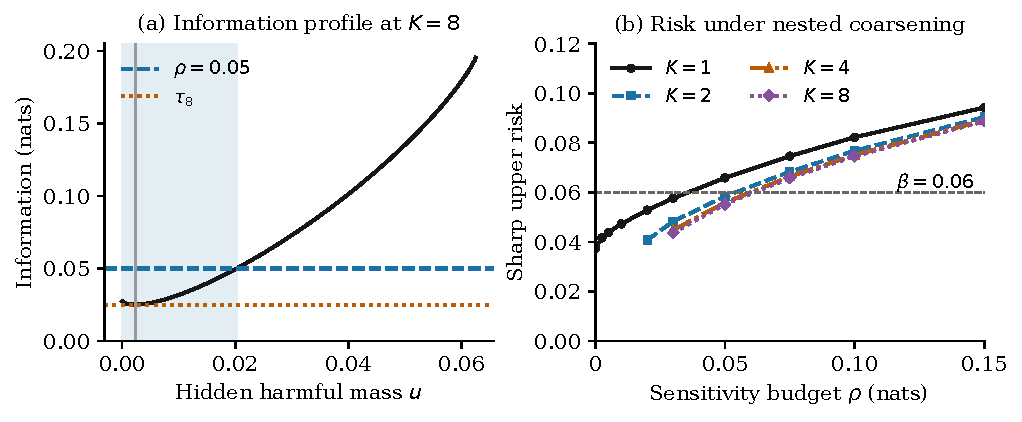
\includegraphics[width=\linewidth]{figures/identification.pdf}
\caption{Population information geometry for the timing-and-terminal harmful-late law ($\theta=0.05$, $q_1=0.30$, $q_0=0.05$, $\lambda_1=0.45$, $\lambda_0=-0.15$). (a) Eight-band information profile on a 1,001-point grid. Shading marks the compatible hidden masses at $\rho=0.05$; the vertical line marks $\ud$. (b) Sharp upper risks at the evaluated sensitivity budgets, under nested coarsenings of one eight-band law. The horizontal line is $\beta=0.06$. Incompatible values are absent; joining segments guide the eye and are not additional evaluations.}\label{fig:identification}
\end{figure}

\FloatBarrier

\section{Anytime-valid risk certification}\label{sec:sequential}
\subsection{Maturation and the observable confidence sequence}
An event enters inference once, when its age reaches $H$, even if its label was resolved earlier. Its category is then permanent. This avoids selecting earlier statistical observations merely because they resolve faster. Let $Y_1,Y_2,\ldots$ denote the categories in this maturity order, with filtration $\mathcal F_n$. Assume that there is one fixed categorical law $p$ such that
\begin{equation}\label{eq:stable}
 \Ebb[\ind\{Y_n=j\}\mid\mathcal F_{n-1}]=p_j
 \quad\text{for every category }j\text{ and every }n.
\end{equation}
Independent identically distributed categorical observations satisfy this assumption. A fixed policy, verification regime, horizon and label semantics define the stable stream to which a certificate applies. Equation~\eqref{eq:stable} does not cover arbitrary drift or arbitrary informative reordering.

The target risk $\theta$ and unresolved harmful mass $u$ refer to one fixed full law of matured events. Equation~\eqref{eq:stable} additionally specifies the conditional stability of the observable categories needed for sequential inference. Stability of the observed categories alone does not identify a changing latent risk.

Write $S_{j,n}=\sum_{i\le n}\ind\{Y_i=j\}$. For $x\in(0,1)$, the per-category Jeffreys mixture likelihood ratio is
\begin{equation}\label{eq:mixture}
 M_{j,n}(x)=\frac{B(S_{j,n}+1/2,n-S_{j,n}+1/2)}
 {B(1/2,1/2)x^{S_{j,n}}(1-x)^{n-S_{j,n}}},
\end{equation}
where $B$ is the beta function. Define raw intervals as the closures of $\{x:M_{j,n}(x)<d/\delta\}$, take their running intersections over all prefixes, and intersect their product with the probability simplex:
\begin{equation}\label{eq:CS}
 \Cset_n=\{p\in\mathbb R_+^d:\sum_jp_j=1,
              \ \ell_{j,n}\le p_j\le v_{j,n}\text{ for every }j\}.
\end{equation}
The construction allocates $\delta/d$ per category and gives
\begin{equation}\label{eq:CSguarantee}
 \Pbb\{p\in\Cset_n\text{ for every }n\}\ge1-\delta.
\end{equation}
The mixture-martingale and maximal-inequality arguments follow established confidence-sequence principles \citep{howard2021,ramdas2023}. The coordinatewise construction is used because its intervals admit simple aggregate envelopes; joint multinomial regions provide an alternative \citep{lindon2022}.

Endpoint nulls $p_j=0,1$ use their limiting likelihoods. Numerical inversion returns the outer endpoints of root brackets, not their midpoints. The region is updated at every matured event, even when risk optimization is performed only at selected checkpoints.

\subsection{Conservative projection and computation}
The ideal upper-risk projection is
\begin{equation}\label{eq:idealprojection}
 U_n^{\rm exact}(\rho)=\sup_{p'\in\Cset_n}\sup\Thset(p',\rho),
\end{equation}
where incompatible $p'$ contribute no risks. An empty feasible union produces no certificate. This is a confidence projection of the identified set, not a plug-in estimate of its upper endpoint.

The implementation first encloses all observable summaries from $\Cset_n$ in an aggregate envelope. Direct category sums and complementary sums give simultaneous intervals for $A,G,c$. In particular,
\begin{equation}\label{eq:aggregate}
 A_L=\max\Big\{\sum_k\ell_{a_k},\ 1-\sum_kv_{b_k}-v_c,\ 0\Big\},\quad
 A_U=\min\Big\{\sum_kv_{a_k},\ 1-\sum_k\ell_{b_k}-\ell_c,\ 1\Big\},
\end{equation}
with analogous formulas for $G$ and $c$. By coordinatewise monotonicity of $q(a,b)$,
\begin{align}
 T_L&=\sum_k q(\ell_{a_k},\ell_{b_k}),\label{eq:entropyenv}\\
 T_U&=\min\left\{\sum_kq(v_{a_k},v_{b_k}),\
 \min\big(1,\sum_k(v_{a_k}+v_{b_k})\big)\log2,\ \log2\right\}.\nonumber
\end{align}
Thus $\Eset_n=\{(A,G,T):A\in[A_L,A_U],G\in[G_L,G_U],1-A-G\in[c_L,c_U],T\in[T_L,T_U]\}$ contains every true summary on the event in \eqref{eq:CSguarantee}. It may contain combinations unattainable by a categorical law. Maximizing over this envelope is a deliberate relaxation.

Because the information constraint decreases in $T$, the relaxed upper projection sets $T=T_U$ and searches over $(A,G,u)$:
\begin{equation}\label{eq:relaxedprojection}
 V_n(\rho)=\sup\left\{A+u:
 \begin{array}{l} A\in[A_L,A_U],\ G\in[G_L,G_U],\ c=1-A-G\in[c_L,c_U],\\
 0\le u\le c,\ h(A+u)-T_U-q(u,c-u)\le\rho
 \end{array}\right\}.
\end{equation}
A nonempty feasible union in \eqref{eq:idealprojection} is contained in this relaxation. The numerical search is designed to upper-bound the relaxation $V_n$. The time-uniform guarantee applies when the reported bound is a conservative enclosure, as required by Theorem~\ref{thm:anytime}.

Deterministic branch-and-bound uses boxes in three aggregate coordinates. A box is discarded only if its geometric constraints are impossible or a lower enclosure of the information exceeds $\rho$. Every remaining box contributes its objective upper bound $\min(1,A_{\rm hi}+u_{\rm hi})$ to the global bound. Candidate feasible joint tables supply lower incumbents, not certificates. Entropy enclosures use Arb ball arithmetic at 128 bits \citep{johansson2017}. The revised implementation uses directed mass and objective arithmetic, interval-verified likelihood-ratio signs, outward summary metadata and conservative singleton brackets. The Supplement gives a source-level enclosure argument for the confidence inversion, projection, feasible witnesses and both rejection searches, under the stated arithmetic and execution assumptions. The archived experiments predate these numerical repairs; their saved decisions are empirical results, without a new end-to-end numerical certification. The uncertainty of the global entropy envelope need not shrink within a search box, so a small box does not imply a small objective gap.

The computation returns the largest retained upper bound on node exhaustion, stall, box-resolution termination or conservative arithmetic fallback. Objective convergence is recorded only when the upper-minus-incumbent gap meets the declared tolerance. Decision-targeted search can stop once the global upper bound is at most $\beta$, or once a candidate feasible risk exceeds $\beta$. With a numerically verified feasible incumbent, the latter justifies withholding certification; it does not show that the true risk exceeds $\beta$. Full derivations and the bounding invariant appear in the Supplement.

\begin{theorem}[Time-uniform sensitivity certificate]\label{thm:anytime}
Suppose \eqref{eq:stable} holds, the true full law satisfies \eqref{eq:pis}, and each reported numerical bound conservatively encloses the projection described above. For a fixed analysis partition and its per-category allocation,
\begin{equation}\label{eq:anytime}
 \Pbb\{\theta\le\widehat U_n(\rho)\text{ at every valid reported update }n\}\ge1-\delta.
\end{equation}
Consequently, for any monitoring rule that issues a certificate only when $\widehat U_n(\rho)\le\beta$, the probability of ever certifying when $\theta>\beta$ is at most $\delta$.
\end{theorem}
\begin{proof}
For the true $p_j\in(0,1)$, \eqref{eq:mixture} is a nonnegative mixture martingale of initial value one under \eqref{eq:stable}; at boundary probabilities the limiting process is a nonnegative supermartingale. The maximal inequality and a union bound give \eqref{eq:CSguarantee}. On this single simultaneous event, the true observable summary and true terminal completion are feasible for every projection. Data processing makes the coarse information no greater than $\rho$. The projected and numerical upper bounds therefore dominate $\theta$ at all reported times. A false certificate requires leaving that simultaneous event.
\end{proof}

The statement is per prespecified partition. Comparing four partitions in a simulation does not allocate a joint four-partition error budget. Choosing a partition from the same data and issuing whichever certificate is most favorable requires a simultaneous allocation across those procedures or a common finest-law region. Likewise, the theorem concerns monitoring within one stable stream, not a familywise guarantee over many streams.

\subsection{Decision states}
After data and numerical validity checks, the implemented evidence gate requires at least 200 matured and 50 resolved events. It then assigns, in order: \emph{model incompatible} if a conservative lower bound on every plausible compatibility floor exceeds $\rho$; \emph{intrinsically uncertifiable} if a conservative lower bound on every compatible minimum-information risk exceeds $\beta$; \emph{certified} if $\widehat U_n\le\beta$; and \emph{uncertified} otherwise. Count shortfalls give \emph{insufficient evidence}. The strong intrinsic state is withheld if zero resolved population mass remains plausible. The first two rejections require conservative numerical lower bounds; comparison guards alone do not establish that contract.

An empty running confidence region is a realized confidence-sequence failure event. The affected procedure stops issuing updates; the stream remains in the simulation denominator. It is not replaced by another seed. A technical execution failure is different from any of these scientific states. No state asserts that compatibility has verified the unobserved sensitivity assumption.

\section{Experimental design}\label{sec:design}
\subsection{Synthetic laws and matched information comparisons}
All primary evidence is synthetic, so the harmful prevalence and full joint law are known. At the finest resolution $K^*=8$, conditional band probabilities are
\begin{equation}\label{eq:law}
 w_k(\lambda)=\frac{\exp\{\lambda(k-(K^*+1)/2)\}}
 {\sum_{j=1}^{K^*}\exp\{\lambda(j-(K^*+1)/2)\}},\qquad
 \Pbb(J^*=k\mid L=\ell)=(1-q_\ell)w_k(\lambda_\ell),
\end{equation}
with $\Pbb(J^*=\infty\mid L=\ell)=q_\ell$ and $L\sim\operatorname{Bernoulli}(\theta)$. Positive $\lambda$ shifts resolved mass later. Analyses at $K=1,2,4,8$ merge adjacent bands of the same finest law; they do not regenerate a different timing distribution. Terminal age is fixed at eight synthetic time units.

\begin{table}[!htbp]\centering
\caption{Principal generating laws. The strong-timing law and matched control share $\theta,q_1,q_0$, hence identical endpoint masses. Additional validity and boundary laws are specified in the Supplement.}\label{tab:laws}
\begin{tabular}{lrrrrr}\toprule
Law & $\theta$ & $q_1$ & $q_0$ & $\lambda_1$ & $\lambda_0$\\\midrule
Timing and terminal, harmful late & .05 & .30 & .05 & .45 & -.15\\
Strong timing & .02 & .30 & .20 & 1.50 & -.60\\
Matched no timing & .02 & .30 & .20 & 0 & 0\\
Low prevalence & .01 & .30 & .05 & .45 & -.15\\
Independent resolution & .05 & .10 & .10 & 0 & 0\\\bottomrule
\end{tabular}
\end{table}

The population decision study crosses six laws, 15 sensitivity budgets, four partitions and six risk budgets. It therefore contains 90 law--sensitivity cells, 360 distinct partition-specific risk profiles, and 2,160 decision rows. Each compatible production upper endpoint is compared with an independent direct-information oracle. The oracle evaluates the full contingency-table information at 100 decimal digits, locates its minimum without the production profile solver, and brackets the admissible endpoints. This checks numerical agreement, separately from the analytical sharpness proof.

\subsection{Prespecified certification-power evaluation}
The confirmatory power design contains 13 scenarios and 32 scenario--partition cells, each with 100 independent event streams. The strong-timing law was selected by a population-feasibility search to exhibit a substantial timing advantage. Its matched null removes only the timing slopes. The local design record fixes the laws, budgets, partitions and checkpoint grids on 19 October 2026, before the original confirmatory evaluation. The completed records analyzed here retain those choices and stream indices; execution batch sizes changed subsequently (Section~\ref{sec:provenance}). Exploratory indices were below 1,000,000; confirmatory indices are 1,000,000--1,000,099. Within a law, partition comparisons reuse the same finest-resolution event streams. Thus streams are independent within a cell, but cells sharing streams are not independent replications.

Separate exploratory stream pilots informed the checkpoint horizons and comparator inclusion before the confirmatory evaluation. These pilots used disjoint stream indices and were not pooled with the 100-stream confirmatory samples. In particular, the 50,000-event strong-timing horizon and the computationally constrained matched-control comparisons were selected during this exploratory phase. The reported certification proportions use only the prespecified confirmatory streams.

At every matured event, the procedure updates its categorical confidence sequence and records exclusion of the known true observable law. It computes risk decisions at prespecified checkpoints. The strong-timing and matched-control grids are 2,000, 5,000, 10,000, 20,000 and 50,000; the endpoint-uncertifiable comparison uses 10,000, 20,000 and 50,000. Low prevalence uses 500, 1,000, 2,000, 5,000, 10,000 and 20,000. Other grids and all final-cell outcomes appear in the Supplement. All sample horizons count matured events, rather than elapsed calendar time. The error level is $\delta=0.05$ for each fixed partition. The population class and its certification margin are determined before generating the streams.

The primary power statistic is the proportion of all 100 streams that have ever certified by a checkpoint, with exact two-sided 95\% Clopper--Pearson intervals \citep{clopper1934}. These intervals describe Monte Carlo uncertainty about certification probability; they are not intervals for $\theta$. First-certification times are checkpoint times, with administrative right-censoring at the horizon. No-certification streams are retained. A stopped empty-region path contributes no later updates but remains in the ever-certified denominator. The prespecified final-horizon power target is met when the lower exact limit is at least 0.8 for a population-certifiable cell. No inference treats repeated looks as independent observations. Intervals are conditionwise, without across-cell multiplicity adjustment.

\subsection{Validity, comparators and numerical cost}
The separate validity study retains seven scenarios, each with 500 independent streams of 500 matured events, and risk checkpoints every 100 events. It checks the categorical construction and its risk projection, including a 32-band law and a minimum-information completion. Exact one-sided 95\% binomial upper limits for ever-violation probabilities are compared with the configured acceptance limit 0.06. The theoretical error guarantee remains 0.05. This horizon is used for validity diagnostics, not certification power.

The principal comparator is endpoint-only TrajCert with the same $\rho$, risk budget, stream and time-uniform construction. Two additional references answer different questions. Repeated-static monitoring projects Bonferroni-adjusted per-category Wilson intervals afresh at each checkpoint, using the same sensitivity model and numerical optimization. It has no time-uniform guarantee; its finite-sample fixed-time coverage is also approximate. The ignorable-delay reference applies a Bernoulli mixture confidence sequence to the resolved labels and uses stronger identification assumptions; it is interpreted as applicable only on laws with $q_1=q_0$ and $\lambda_1=\lambda_0$. Assumption-violated runs are diagnostics, not evidence of superiority over a valid comparator.

Numerical validation includes direct-oracle comparisons, theorem-identity checks and an independent feasible-risk check on stored finite-sample envelopes. Scaling uses $K=1,2,4,8,16,32,64,128$, five warmups and 30 measured invocations per target in isolated processes with numerical-library thread limits set to one. Each $K$ regenerates the specified conditional-law form for this computational benchmark and uses its own true information plus 0.01 nats, outside the timed region. Thus this is a cost benchmark, not a nested-refinement experiment. The outer target includes the generation and sequential processing of a deterministic 500-event balanced-prefix ledger and its final projection, so its runtime is broader than the isolated optimizer call. The software is Python with NumPy, SciPy, mpmath and python-flint; exact dependency locks accompany the repository. The completed benchmark does not record enough hardware information for a portable speed claim.

\subsection{Evidence provenance}\label{sec:provenance}
The results use the latest completed records, their completion markers and the corresponding report exports. Every checkpoint certification count and exact binomial interval was reconstructed from individual stream outcomes. The current campaign contains 3,200 single-stream power batches and 3,500 single-stream validity batches. Relative to the retained design copy, the only configuration changes are execution batch sizes: ten to one for power and fifty to one for validity. Laws, budgets, stream indices and evaluation grids are unchanged. The original design is locally documented rather than independently preregistered.

All 116 rendered source/destination pairs in the current report match their recorded hashes. The final power-summary table agrees with the previous publication archive, while checkpoint runtimes and numerical gaps differ. The runtime results below therefore use the current records exclusively. Dependency fingerprints cover the configuration, dependency locks and parent artifacts but omit a source-tree digest; the report commit identifies the reporting checkout and does not attest the exact implementation used by every stream. The Supplement supplies the current and frozen configuration hashes, completion-record identity and a checksummed archive of the evidence used here.

This manuscript revision recalculated summaries and publication assets without changing scientific records or executing experiments.

\section{Results}\label{sec:results}
\subsection{Sharpness and numerical reliability}
The population-solver validation comprises 280 cases: 14 laws at each combination of four partitions and five information-offset levels. Every state comparison agrees with the independent oracle. The largest absolute upper-risk discrepancy is $4.615\times10^{-13}$. Over the 360 partition profiles in the decision study, the largest discrepancy is $4.002\times10^{-13}$. These are numerical checks of the computed endpoints; sharpness itself follows from Theorem~\ref{thm:sharp}.

All 54 partition-coherence cases satisfy nesting, and the 18 strict-timing cases and 24 same-endpoint timing cases pass their specified checks. Recorded checks of profile decomposition, curvature, the compatibility floor and constructive completions support consistency of the implementation with the analytical identities. An independent finite-sample feasible-risk check yields 33 comparable envelopes among 40 cases, with no reported upper bound below the oracle feasible-risk diagnostic; seven cases have no oracle feasible point and provide no directional comparison. Decision-targeted and full searches agree on all 176 recorded budget comparisons. Such finite validation cannot certify all floating-point executions, but it supports the intended conservative search invariant.

\subsection{Timing changes population certification decisions}
Table~\ref{tab:population} gives a common-budget comparison for the timing-and-terminal harmful-late law. At $\rho=0.05$, every displayed partition is compatible. Endpoint information gives an upper risk of $0.065835$, exceeding $\beta=0.06$. Two bands suffice to cross the decision threshold, and further refinement lowers the upper endpoint to $0.055241$ at eight bands. The observed outcome and terminal-selection marginals are identical across these analyses.

\begin{table}[!htbp]\centering
\caption{Population decision value at $\rho=0.05$ and $\beta=0.06$ for the timing-and-terminal harmful-late law. Information quantities are in nats. A decision is a sharp population statement, without sampling uncertainty.}\label{tab:population}
\begin{tabular}{rrrrl}\toprule $K$ & $\tau_K$ & $\theta_{U,K}(0.05)$ & $\rho_K^*(0.06)$ & Decision\\\midrule
1 & 0.000000 & 0.065835 & 0.035491 & Uncertified\\
2 & 0.018323 & 0.058346 & 0.053814 & Certified\\
4 & 0.023710 & 0.055899 & 0.059201 & Certified\\
8 & 0.025106 & 0.055241 & 0.060597 & Certified\\\bottomrule\end{tabular}

\end{table}

The complete-case risk is $\td=0.037333$ and the assumption-free upper bound is $A+c=0.0975$. The eight-band compatibility floor is $0.025106$. Timing raises the certification frontier at $\beta=0.06$ from $0.035491$ at the endpoint to $0.060597$ at eight bands. The frontier difference, $0.025106$ nats, is exactly the observable timing increment. Hence, at this risk budget, the eight-band analysis changes the decision for $\rho$ in approximately $(0.035491,0.060597]$; this window lies above its compatibility floor. Figure~\ref{fig:identification} connects the profile to this sensitivity comparison.

The sensitivity budget can also be interpreted through the admissible harmful proportion among unresolved events. For the law in Table~\ref{tab:population}, the resolved harmful proportion is $A/r=0.0373$. At $\rho=0.05$, the endpoint upper-risk completion permits an unresolved harmful proportion of approximately 0.493, compared with 0.324 for eight timing bands. Relative to the resolved proportion, the corresponding harmful-outcome odds ratios are approximately 25.1 and 12.4. These quantities describe worst-case completions admitted by the assumed information budget, not estimates of the actual unresolved-outcome mechanism.

Across all 2,160 decision rows, 34 change from endpoint noncertification to refined certification: 13 for the timing-and-terminal law, 11 for high unresolvedness and 10 for timing-only selection. These are counts within a fixed design grid, not estimated probabilities of benefit. The no-path-dependence, terminal-only and low-prevalence controls produce no decision changes on this grid. At eight bands, the ordinary harmful-late law at $\rho=0.05,\beta=0.06$ remains a small-margin example: its separate confirmatory power evaluation certifies 0/100 streams by 20,000 events, as does the endpoint analysis. Its decision value is established at the population level; the next experiment addresses finite-sample value on a different, stronger-timing law.

\subsection{Finite-sample certification under informative timing}
The strong-timing law has true risk $0.02$. At $\rho=0.08$, its sharp population upper risks are $0.079617$, $0.059129$, $0.049755$ and $0.047196$ for $K=1,2,4,8$, respectively. At $\beta=0.09$, all are population-certifiable, but their margins and statistical dimensions differ substantially.

Figure~\ref{fig:power}(a) and Table~\ref{tab:power} show the resulting certification probabilities. The two-band procedure certifies 100/100 streams by 5,000 matured events, with exact 95\% interval $[0.964,1]$. Endpoint-only analysis certifies none by 5,000 and 96/100 by 50,000, with interval $[0.901,0.989]$. The 5,000-event horizon is one tenth of the 50,000-event horizon in this descriptive comparison of high observed certification frequencies. It is not a universal tenfold sample-complexity result. Four bands certify 88/100 by 5,000 and 100/100 by 10,000; eight bands certify 98/100 by 10,000. Intermediate resolution certifies earlier here, although eight bands give the smaller population bound.

The early difference is not explained solely by incomplete optimization. At 5,000 events, endpoint decision-targeted searches refuted certification in 89 of 96 streams and remained numerically unresolved in seven. The two-band procedure certified all 100 streams. At later checkpoints, unresolved numerical searches also contribute to delayed certification. The four full-search representatives are included in the headline totals but not in this targeted-search decomposition.

\begin{figure}[!htbp]
\centering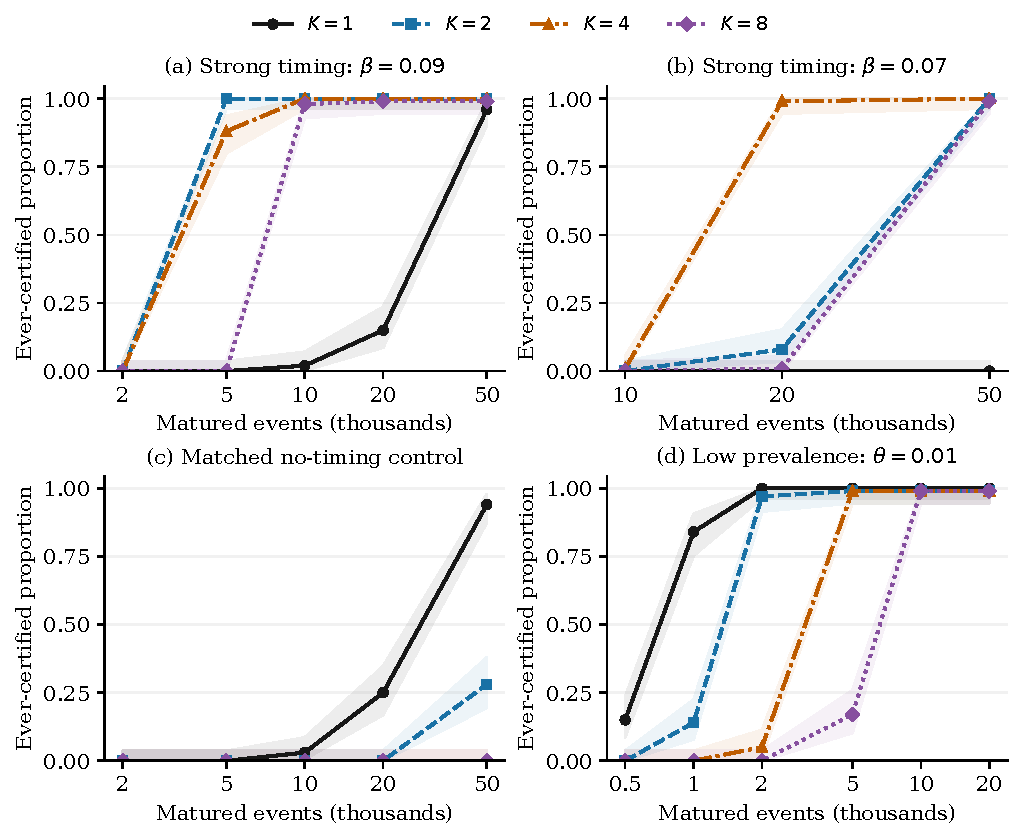
\includegraphics[width=\linewidth]{figures/certification_power.pdf}
\caption{Confirmatory certification by checkpoint, using 100 independent streams per scenario--partition cell and $\delta=0.05$ per fixed partition. Lines join observed ever-certified proportions; shaded bands are conditionwise exact two-sided 95\% Clopper--Pearson intervals. (a) Strong timing, $\rho=0.08,\beta=0.09$. (b) The same law and $\rho$, with $\beta=0.07$, below the endpoint population upper bound. (c) Matched endpoint masses with no timing contrast, $\rho=0.08,\beta=0.09$. (d) Low-prevalence law, $\rho=0.02,\beta=0.05$. Partition analyses within a law share finest-resolution streams. Checkpoints within a stream are dependent.}\label{fig:power}
\end{figure}

\begin{table}[!htbp]\centering
\caption{Selected strong-timing certification results at $\rho=0.08$. Counts refer to ever certifying by the stated horizon. Intervals quantify Monte Carlo certification probability across 100 streams, separately for each row. The full checkpoint curves and matched control are in Figure~\ref{fig:power}.}\label{tab:power}
\begin{tabular}{rrrrl}\toprule $\beta$ & $K$ & Horizon $n$ & Certified streams & Exact 95\% interval\\\midrule
0.09 & 1 & 50,000 & 96/100 & [0.9007, 0.9890]\\
0.09 & 2 & 5,000 & 100/100 & [0.9638, 1.0000]\\
0.09 & 4 & 5,000 & 88/100 & [0.7998, 0.9364]\\
0.09 & 4 & 10,000 & 100/100 & [0.9638, 1.0000]\\
0.09 & 8 & 10,000 & 98/100 & [0.9296, 0.9976]\\
0.07 & 1 & 50,000 & 0/100 & [0.0000, 0.0362]\\
0.07 & 2 & 50,000 & 100/100 & [0.9638, 1.0000]\\
0.07 & 4 & 20,000 & 99/100 & [0.9455, 0.9997]\\
0.07 & 8 & 50,000 & 99/100 & [0.9455, 0.9997]\\\bottomrule\end{tabular}

\end{table}

At the stricter $\beta=0.07$, the endpoint model is compatible but its sharp upper bound exceeds the budget. The trajectory partitions remain population-certifiable. Endpoint analysis certifies 0/100 through 50,000 events, while $K=2$ certifies 100/100 by 50,000, $K=4$ certifies 99/100 by 20,000 and 100/100 by 50,000, and $K=8$ certifies 99/100 by 50,000. Thus the comparison changes both the population decision and its finite-sample realization. Endpoint population noncertifiability is a statement about the identified set; a stochastic procedure can still issue an erroneous certificate on its confidence failure event.

The low-prevalence study provides a complementary nonvacuity check at $\theta=0.01,\rho=0.02,\beta=0.05$. Endpoint analysis certifies 100/100 by 2,000 events, two bands 97/100 by 2,000, four bands 99/100 by 5,000 and eight bands 99/100 by 10,000. Here the endpoint already has a large certification margin, so refinement does not improve the required horizons.

\subsection{When resolution pays for its statistical cost}
The matched no-timing law preserves the strong-timing law's endpoint masses but has no resolved timing information. All four population upper bounds equal $0.079617$. At 50,000 events, the certification counts are 94/100, 28/100, 0/100 and 0/100 as $K$ increases from one to eight (Figure~\ref{fig:power}c). Without informative timing, finer partitions yield lower certification frequencies in this matched control. The observed cost reflects the combined effects of categorical sampling uncertainty, aggregate-envelope relaxation and incomplete numerical search. At 50,000 events, the two-band decision-targeted searches comprise 27 current certificates, one refutation, 67 unresolved searches and one stopped path among 96 streams. The eight-band targeted searches comprise 94 refutations and two stopped paths. The four full-search representatives are accounted for separately in the reported 100-stream certification totals (Supplement). Theorem~\ref{thm:refinement} concerns population identification; it does not order finite-sample envelopes constructed with different category counts.

The additional references expose a separate trade-off. For the low-prevalence endpoint analysis at 500 events, repeated-static monitoring certifies 71/100 compared with 15/100 for TrajCert; at 1,000, the counts are 99/100 and 84/100. This power advantage comes without the time-uniform guarantee. The dense-monitoring comparison records no certification by either procedure at its risk budget; it does not demonstrate optional-stopping failure of repeated-static monitoring. In the ignorable-delay valid regime, the reference certifies 98/100 by 20,000 events; TrajCert certifies 98/100 at $K=1$ and 0/100 at $K=8$. Its stronger identification assumption explains why the reference need not pay the same sensitivity cost. Full outcomes, including noncertifying controls, are reported in the Supplement.

\subsection{Time-uniform validity diagnostics}
Table~\ref{tab:coverage} summarizes the seven retained validity scenarios. TrajCert's recorded violation diagnostic counts either an empty running region or a reported risk upper bound below the known risk. Its counts agree with the categorical-construction counts in these artifacts: one stream in the independent-resolution control, one in high unresolvedness, and none in the other five scenarios. Both nonzero diagnostics arise from empty running regions. The exact one-sided upper limits are $0.00945$ for 1/500 and $0.00597$ for 0/500, both below the configured 0.06 acceptance limit. All seven cells complete without technical failure. These conditionwise checks are consistent with the theorem but neither prove it nor establish a simultaneous 95\% campaign-level coverage statement. No scenario certifies within 500 events; certification power is evaluated separately above.

\begin{table}[!htbp]\centering
\caption{Time-uniform validity diagnostics through 500 matured events per stream, with risk projections at 100-event checkpoints. Each scenario has 500 independent streams. Limits are exact one-sided 95\% limits for the recorded ever-violation event, separately by scenario. The configured acceptance limit is 0.06, while the nominal theoretical level is $\delta=0.05$.}\label{tab:coverage}
\begin{tabular}{lrrr}\toprule Scenario & $K$ & Violations / streams & One-sided 95\% upper\\\midrule
High unresolvedness & 8 & 1/500 & 0.00945\\
Independent resolution & 8 & 1/500 & 0.00945\\
Low prevalence & 8 & 0/500 & 0.00597\\
Minimum-information completion & 8 & 0/500 & 0.00597\\
Near certification boundary & 8 & 0/500 & 0.00597\\
Near degeneracy & 8 & 0/500 & 0.00597\\
Thirty-two bands & 32 & 0/500 & 0.00597\\\bottomrule\end{tabular}

\end{table}

No false risk certification is recorded in any of the 32 power cells; zero of 100 gives a one-sided 95\% upper limit of $0.02951$ per cell. No cell with a compatible population model and a sharp upper risk above $\beta$ records a certificate. This does not imply zero error probability. Confidence-sequence exclusions of the true law range from one to six of 100 by cell, illustrating why validity is probabilistic. In the deliberately incompatible-budget cell at $K=4$, 16/100 streams certify by 20,000 even though the sensitivity assumption is false; their true risk is below $\beta$, so they are not counted as false risk certifications. No model-incompatible state was reported at the tested checkpoints, including in the two incompatible-budget cells. The finite-sample incompatibility check therefore did not detect those budget violations at the evaluated horizons. Its failure to reject cannot establish that the declared sensitivity restriction holds. These cases are retained in the Supplement and excluded from claims under a correctly specified sensitivity model.

\subsection{Computation and sensitivity boundaries}
Figure~\ref{fig:computation} separates the two computational scales. Population median runtimes are $0.419$--$0.466$ ms over $K=1$--128, with a reported median of 36 total root iterations at every $K$. Oracle discrepancies in this benchmark do not exceed $3.592\times10^{-13}$. The broader 500-event outer-projection target takes median $1.027$--$7.546$ seconds, with peak process resident memory $210.82$--$214.65$ MiB. These process-memory measurements include the Python runtime and libraries. Finite-sample projection is substantially more expensive than the scalar population solve; a conservative early return can also be less tight than the optimization target. Neither the runtime benchmark nor a node cap establishes a worst-case complexity bound for the projection.

The power-study checkpoints provide an additional operational cost measure. Across the 160 recorded checkpoint-level runtime medians, the median is 0.922 s and the maximum is 31.004 s; eleven checkpoint medians exceed 10 s. These timings exclude the four full-search representatives per cell and cover checkpoint projection-related computation rather than complete stream processing. They are distinct from the isolated scaling benchmark, and the available hardware record does not support a portable runtime comparison.

\begin{figure}[!htbp]
\centering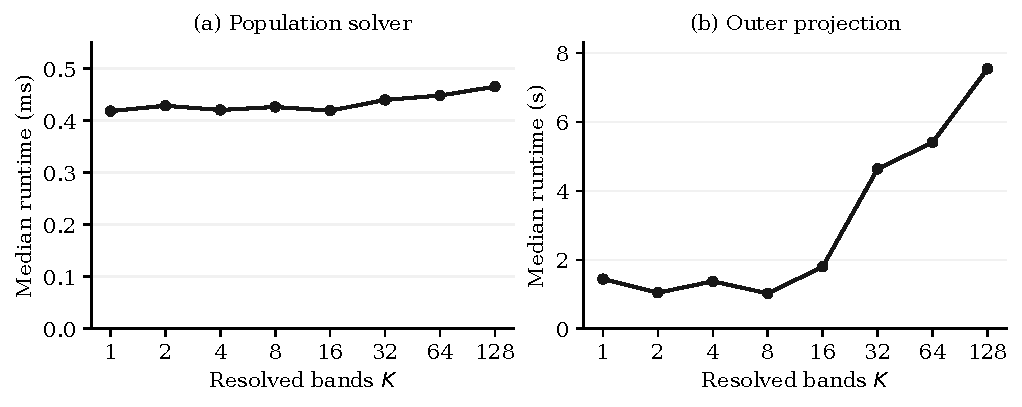
\includegraphics[width=\linewidth]{figures/computation.pdf}
\caption{Computational benchmark from existing records: medians of 30 isolated measured invocations after five warmups per $K$, with numerical-library threads limited to one. (a) Population solver, including law and summary construction. (b) Broader outer target, including a deterministic 500-event ledger, sequential confidence updates and the final projection. The law form is regenerated at each $K$, and both targets use its true information plus 0.01 nats. These curves measure cost, not nested-law information gain.}\label{fig:computation}
\end{figure}

The compatibility and risk frontiers explain the sensitivity regimes without an additional estimator. At fixed observed margins, increasing $\rho$ widens the admissible risk interval. At fixed $\rho$, refinement can either tighten a compatible interval or reveal incompatibility. An expected-count diagnostic for the low-prevalence law at $\rho=0.02,\beta=0.05$ gives upper bounds $0.0540$ at 5,000 and $0.0404$ at 10,000 events. This deterministic illustration locates a transition between those sizes; it is not a Monte Carlo estimate of certification probability.

\FloatBarrier

\section{Discussion}\label{sec:discussion}
The observation process has two roles in this problem. Nonresolution creates an unidentified terminal harmful mass, while the resolved path supplies an observable information requirement. The profile decomposition separates these roles: $\tau_\Pi$ accounts for dependence already observed in resolved timing, leaving a smaller allowance for terminal selection. Coarsening removes part of that observable requirement, leaving more dependence available to adverse terminal completions. This accounts for the larger endpoint risk set under a common budget.

The exact frontier $\rho_\Pi^*(\beta)$ provides a direct sensitivity report. It identifies the budgets at which a particular risk decision follows from the observed law, together with the budgets ruled out by compatibility. Its shift under refinement is the same conditional information that appears in the profile identity. The population decision example and the endpoint-uncertifiable power scenario give two realizations of this geometry, at different risk and information budgets.

Finite-sample resolution is a design choice with a cost. The strongest timing law supports markedly earlier certification with two bands, whereas its matched null favors endpoint-only inference. Additional timing bands can tighten the population bound while increasing confidence-region uncertainty and numerical relaxation. These findings support choosing a prespecified resolution appropriate to the expected timing structure; they do not support selecting the most favorable certificate after inspecting multiple unadjusted analyses.

The present guarantees concern trustworthy labels and event records, a fixed terminal horizon, a stable categorical law, and a sensitivity assumption that holds for the target stream. The experiments demonstrate the mechanism on designed synthetic laws. They do not estimate its prevalence across applications or establish a portable calibration of $\rho$. Richer joint confidence regions, tighter projection envelopes and application-specific sensitivity elicitation are natural questions, but changes to these components would require their own validation. The current computational contribution is a transparent conservative implementation with traceable numerical evidence, rather than a finite-sample optimality claim.

\section{Conclusion}\label{sec:conclusion}
Under a mutual-information constraint on a categorical outcome-resolution path, latent harmful risk has a sharp interval characterized by one scalar completion. Observable timing information determines the compatibility floor and shifts the risk-certification frontier exactly under refinement. Projecting a simultaneous observable-law confidence sequence through this model gives an anytime-valid certificate with conservative numerical computation. The verified experiments show both consequences of retaining timing: decisions unavailable to an endpoint population analysis, and high finite-sample certification at substantially shorter horizons under informative timing. The matched control identifies the condition behind that benefit: timing must add enough relevant information to offset the statistical cost of observing it at finer resolution.

\section*{Declarations}
\paragraph{Code and data availability}
All primary results use synthetic laws specified in the article and Supplement. Code, configuration, dependency locks and exported numerical source data are publicly available at \url{https://github.com/naslouby-salahe/TrajCert}, with the local source inspected at commit \texttt{e4f5cef47d3af18f5badcb0a644dbc3636d52cd5}. The supplementary archive \texttt{evidence\_current.zip} supplies the numerical sources used in the article, completion records, confirmatory stream outcomes, validity batches, configuration and dependency locks with checksums. No permanent archive DOI or release tag is asserted. The optional external diagnostic dataset is not used as evidence in this article.
\paragraph{Competing interests}
The authors declare no competing interests.
\paragraph{Funding}
This research received no specific grant from funding agencies in the public, commercial, or not-for-profit sectors.
\paragraph{Author contributions}
\textbf{Salaheddine Naslouby:} Conceptualization, Methodology, Software, Formal analysis, Validation, Investigation, Visualization, Writing---original draft, Writing---review and editing.
\textbf{Mohamed Lachgar:} Supervision, Writing---review and editing.
\textbf{Hamid Hrimech:} Supervision, Writing---review and editing.

\bibliographystyle{elsarticle-harv}
\bibliography{references}
\end{document}
